\documentclass[12pt,a4paper]{article}

%=============================================================================
% PACKAGES
%=============================================================================
\usepackage[utf8]{inputenc}
\usepackage[T1]{fontenc}
\usepackage{lmodern}
\usepackage{amsmath,amssymb,amsthm,amsfonts}
\usepackage{mathtools}
\usepackage{graphicx}
\usepackage{hyperref}
\usepackage{geometry}
\usepackage{tcolorbox}
\usepackage{tikz}
\usepackage{pgfplots}
\pgfplotsset{compat=1.18}
\usepackage{booktabs}
\usepackage{enumitem}
\usepackage{fancyhdr}
\usepackage{titlesec}

\geometry{margin=1in}

%=============================================================================
% THEOREM ENVIRONMENTS
%=============================================================================
\theoremstyle{definition}
\newtheorem{definition}{Definition}[section]
\newtheorem{example}[definition]{Example}

\theoremstyle{plain}
\newtheorem{theorem}[definition]{Theorem}
\newtheorem{lemma}[definition]{Lemma}
\newtheorem{proposition}[definition]{Proposition}
\newtheorem{corollary}[definition]{Corollary}

\theoremstyle{remark}
\newtheorem{remark}[definition]{Remark}
\newtheorem*{notation}{Notation}

%=============================================================================
% CUSTOM COMMANDS
%=============================================================================
\newcommand{\R}{\mathbb{R}}
\newcommand{\N}{\mathbb{N}}
\newcommand{\norm}[1]{\left\| #1 \right\|}
\newcommand{\abs}[1]{\left| #1 \right|}
\newcommand{\inner}[2]{\left\langle #1, #2 \right\rangle}
\newcommand{\dd}{\,\mathrm{d}}
\newcommand{\grad}{\nabla}
\newcommand{\dive}{\nabla \cdot}
\newcommand{\lapl}{\Delta}
\newcommand{\Lp}[1]{L^{#1}(\Omega)}
\newcommand{\Hp}[1]{H^{#1}(\Omega)}
\newcommand{\Hzero}{H^1_0(\Omega)}
\newcommand{\weakto}{\rightharpoonup}

%=============================================================================
% COLORED BOXES
%=============================================================================
\tcbuselibrary{theorems,skins,breakable}

\newtcolorbox{keyresult}[1][]{
    colback=blue!5!white,
    colframe=blue!75!black,
    fonttitle=\bfseries,
    title={Key Result},
    #1
}

\newtcolorbox{physicalinsight}[1][]{
    colback=green!5!white,
    colframe=green!60!black,
    fonttitle=\bfseries,
    title={Physical Insight},
    #1
}

\newtcolorbox{numericalconnection}[1][]{
    colback=orange!5!white,
    colframe=orange!75!black,
    fonttitle=\bfseries,
    title={Connection to Numerics},
    #1
}

%=============================================================================
% HEADER/FOOTER
%=============================================================================
\pagestyle{fancy}
\fancyhf{}
\fancyhead[L]{\textit{Mathematical Theory of Elliptic PDEs}}
\fancyhead[R]{\textit{Chapter 02}}
\fancyfoot[C]{\thepage}

%=============================================================================
% TITLE
%=============================================================================
\title{
    \vspace{-1cm}
    \textbf{\LARGE Mathematical Foundations of Elliptic PDEs} \\[0.5cm]
    \large Weak Formulation, Functional Analysis, and Variational Principles \\[0.3cm]
    \normalsize Chapter 02 Supplement: Theoretical Foundations
}
\author{
    Computational Physics: Numerical Methods \\
    \small A Rigorous Treatment of Existence, Uniqueness, and Energy Principles
}
\date{\today}

%=============================================================================
\begin{document}
%=============================================================================

\maketitle

\begin{abstract}
This document provides the mathematical foundations for the numerical methods developed in Chapter 02. We present the weak (variational) formulation of elliptic boundary value problems, introduce the essential functional analysis framework (Sobolev spaces, trace theorems), and prove the fundamental Lax-Milgram theorem guaranteeing existence and uniqueness of solutions. We then develop the energy minimization interpretation, showing that solving an elliptic PDE is equivalent to minimizing a quadratic energy functional. Finally, we connect these theoretical concepts to the numerical methods implemented in our code, explaining why Galerkin methods (including finite elements and spectral methods) provide natural discretizations of the weak formulation.
\end{abstract}

\tableofcontents
\newpage

%=============================================================================
\section{Introduction: From Classical to Weak Solutions}
%=============================================================================

\subsection{The Model Problem}

Throughout this document, we consider the Poisson equation with homogeneous Dirichlet boundary conditions as our model problem:

\begin{equation}
\boxed{
\begin{aligned}
    -\lapl u &= f \quad \text{in } \Omega \\
    u &= 0 \quad \text{on } \partial\Omega
\end{aligned}
}
\label{eq:poisson}
\end{equation}

where $\Omega \subset \R^n$ is a bounded, open domain with sufficiently smooth boundary $\partial\Omega$, $f: \Omega \to \R$ is a given source term, and $\lapl u = \sum_{i=1}^n \frac{\partial^2 u}{\partial x_i^2}$ is the Laplacian operator.

\subsection{Limitations of Classical Solutions}

A \textbf{classical solution} requires $u \in C^2(\Omega) \cap C(\overline{\Omega})$ satisfying \eqref{eq:poisson} pointwise. However:

\begin{enumerate}[label=(\roman*)]
    \item Classical solutions may not exist for rough data $f$ or irregular domains
    \item The pointwise interpretation breaks down at corners, interfaces, or singularities
    \item Numerical methods (finite differences, finite elements) naturally produce approximate solutions that are not $C^2$
\end{enumerate}

\begin{physicalinsight}
Consider a membrane deflection problem where a concentrated load (Dirac delta) is applied at a point. The classical formulation $-\lapl u = \delta_{x_0}$ makes no sense pointwise, yet physically the problem has a well-defined solution (a logarithmic singularity in 2D). The weak formulation handles such cases naturally.
\end{physicalinsight}

\subsection{The Key Idea: Integration by Parts}

The transition to weak formulations begins with a simple observation. Multiply \eqref{eq:poisson} by a smooth test function $v$ that vanishes on $\partial\Omega$, and integrate over $\Omega$:

\begin{equation}
    -\int_\Omega (\lapl u) \, v \dd x = \int_\Omega f \, v \dd x
\end{equation}

Applying Green's first identity (integration by parts):
\begin{equation}
    \int_\Omega \grad u \cdot \grad v \dd x - \underbrace{\int_{\partial\Omega} \frac{\partial u}{\partial n} v \dd s}_{=0 \text{ since } v|_{\partial\Omega}=0} = \int_\Omega f \, v \dd x
\end{equation}

This leads to the \textbf{weak formulation}: Find $u$ such that
\begin{equation}
    \int_\Omega \grad u \cdot \grad v \dd x = \int_\Omega f \, v \dd x \quad \forall v \in V
    \label{eq:weak}
\end{equation}

\begin{keyresult}
The weak formulation \eqref{eq:weak} requires only \textbf{first derivatives} of $u$ (not second), allowing solutions in a larger function space. This is the mathematical basis for finite element methods.
\end{keyresult}

%=============================================================================
\section{Functional Analysis Prerequisites}
%=============================================================================

To make the weak formulation rigorous, we need appropriate function spaces.

\subsection{Lebesgue Spaces $L^p(\Omega)$}

\begin{definition}[$L^p$ spaces]
For $1 \leq p < \infty$, we define:
\begin{equation}
    \Lp{p} = \left\{ u: \Omega \to \R \;\Big|\; \int_\Omega |u|^p \dd x < \infty \right\}
\end{equation}
with norm $\norm{u}_{L^p} = \left( \int_\Omega |u|^p \dd x \right)^{1/p}$.

For $p = 2$, $L^2(\Omega)$ is a Hilbert space with inner product:
\begin{equation}
    \inner{u}{v}_{L^2} = \int_\Omega u \, v \dd x
\end{equation}
\end{definition}

\subsection{Sobolev Spaces}

\begin{definition}[Weak derivative]
A function $u \in L^1_{\text{loc}}(\Omega)$ has a \textbf{weak derivative} $\partial_i u = w$ if:
\begin{equation}
    \int_\Omega u \, \partial_i \phi \dd x = -\int_\Omega w \, \phi \dd x \quad \forall \phi \in C^\infty_0(\Omega)
\end{equation}
where $C^\infty_0(\Omega)$ denotes smooth functions with compact support in $\Omega$.
\end{definition}

\begin{definition}[Sobolev space $H^1(\Omega)$]
\begin{equation}
    \Hp{1} = \left\{ u \in \Lp{2} \;\Big|\; \partial_i u \in \Lp{2}, \; i = 1, \ldots, n \right\}
\end{equation}
equipped with the norm:
\begin{equation}
    \norm{u}_{H^1}^2 = \norm{u}_{L^2}^2 + \norm{\grad u}_{L^2}^2 = \int_\Omega \left( u^2 + |\grad u|^2 \right) \dd x
\end{equation}
and inner product:
\begin{equation}
    \inner{u}{v}_{H^1} = \int_\Omega \left( u \, v + \grad u \cdot \grad v \right) \dd x
\end{equation}
\end{definition}

\begin{theorem}[$H^1$ is a Hilbert space]
The Sobolev space $\Hp{1}$ is complete with respect to the $H^1$ norm, hence it is a Hilbert space.
\end{theorem}

\begin{definition}[$H^1_0(\Omega)$: Functions vanishing on the boundary]
\begin{equation}
    \Hzero = \overline{C^\infty_0(\Omega)}^{\norm{\cdot}_{H^1}}
\end{equation}
This is the closure of smooth, compactly supported functions in the $H^1$ norm. Intuitively, these are $H^1$ functions that ``vanish on $\partial\Omega$'' in a generalized sense.
\end{definition}

\subsection{The Poincaré Inequality}

\begin{theorem}[Poincaré inequality]
\label{thm:poincare}
Let $\Omega \subset \R^n$ be a bounded domain. There exists a constant $C_P > 0$ depending only on $\Omega$ such that:
\begin{equation}
    \norm{u}_{L^2} \leq C_P \norm{\grad u}_{L^2} \quad \forall u \in \Hzero
    \label{eq:poincare}
\end{equation}
\end{theorem}

\begin{proof}[Sketch of proof for $\Omega = (0,L)$ in 1D]
For $u \in H^1_0(0,L)$, we have $u(0) = 0$, so:
\begin{equation}
    u(x) = \int_0^x u'(t) \dd t
\end{equation}
By Cauchy-Schwarz:
\begin{equation}
    |u(x)|^2 = \left| \int_0^x u'(t) \dd t \right|^2 \leq x \int_0^x |u'(t)|^2 \dd t \leq L \int_0^L |u'|^2 \dd t
\end{equation}
Integrating in $x$:
\begin{equation}
    \int_0^L |u|^2 \dd x \leq L^2 \int_0^L |u'|^2 \dd x
\end{equation}
Hence $C_P = L$ works. The general proof uses similar ideas with the geometry of $\Omega$.
\end{proof}

\begin{corollary}[Equivalent norm on $H^1_0$]
On $\Hzero$, the seminorm $|u|_{H^1} = \norm{\grad u}_{L^2}$ is equivalent to the full $H^1$ norm:
\begin{equation}
    \norm{\grad u}_{L^2} \leq \norm{u}_{H^1} \leq (1 + C_P^2)^{1/2} \norm{\grad u}_{L^2}
\end{equation}
\end{corollary}

\begin{numericalconnection}
The Poincaré constant $C_P$ depends on the domain size. For $\Omega = (0,L)^n$, we have $C_P \sim L/\pi$. This explains why:
\begin{itemize}
    \item The condition number of the discrete Laplacian grows as $\mathcal{O}(h^{-2})$ when the mesh is refined
    \item Larger domains require more iterations for iterative solvers
    \item Multigrid methods, which coarsen the grid, effectively exploit different Poincaré constants at each level
\end{itemize}
\end{numericalconnection}

%=============================================================================
\section{The Weak Formulation}
%=============================================================================

\subsection{Abstract Setting}

Let $V$ be a Hilbert space. A \textbf{weak formulation} of a PDE has the abstract form:

\begin{equation}
\boxed{
\text{Find } u \in V \text{ such that } a(u, v) = \ell(v) \quad \forall v \in V
}
\label{eq:abstract_weak}
\end{equation}

where:
\begin{itemize}
    \item $a: V \times V \to \R$ is a \textbf{bilinear form}
    \item $\ell: V \to \R$ is a \textbf{linear functional}
\end{itemize}

\subsection{Weak Formulation of the Poisson Equation}

For problem \eqref{eq:poisson}, we set:
\begin{itemize}
    \item $V = \Hzero$
    \item $a(u,v) = \int_\Omega \grad u \cdot \grad v \dd x$ \quad (bilinear form)
    \item $\ell(v) = \int_\Omega f \, v \dd x$ \quad (linear functional, requires $f \in L^2$)
\end{itemize}

\begin{definition}[Weak solution]
A function $u \in \Hzero$ is a \textbf{weak solution} of \eqref{eq:poisson} if:
\begin{equation}
    a(u,v) = \ell(v) \quad \forall v \in \Hzero
    \label{eq:weak_poisson}
\end{equation}
\end{definition}

\begin{theorem}[Classical implies weak]
If $u \in C^2(\Omega) \cap C(\overline{\Omega})$ is a classical solution of \eqref{eq:poisson}, then $u$ is also a weak solution.
\end{theorem}

\begin{proof}
For a classical solution, multiply by any $v \in C^\infty_0(\Omega) \subset \Hzero$ and integrate by parts:
\begin{equation}
    \int_\Omega \grad u \cdot \grad v \dd x = -\int_\Omega (\lapl u) v \dd x = \int_\Omega f v \dd x
\end{equation}
By density of $C^\infty_0$ in $\Hzero$, the equality extends to all $v \in \Hzero$.
\end{proof}

\subsection{Properties of the Bilinear Form}

\begin{definition}[Continuity/Boundedness]
A bilinear form $a: V \times V \to \R$ is \textbf{continuous} (or bounded) if there exists $M > 0$ such that:
\begin{equation}
    |a(u,v)| \leq M \norm{u}_V \norm{v}_V \quad \forall u, v \in V
\end{equation}
\end{definition}

\begin{definition}[Coercivity/Ellipticity]
A bilinear form $a: V \times V \to \R$ is \textbf{coercive} (or $V$-elliptic) if there exists $\alpha > 0$ such that:
\begin{equation}
    a(v,v) \geq \alpha \norm{v}_V^2 \quad \forall v \in V
\end{equation}
\end{definition}

\begin{proposition}
For the Poisson problem with $V = \Hzero$ and $a(u,v) = \int_\Omega \grad u \cdot \grad v \dd x$:
\begin{enumerate}
    \item $a$ is \textbf{symmetric}: $a(u,v) = a(v,u)$
    \item $a$ is \textbf{continuous} with $M = 1$ (using the $H^1$ seminorm)
    \item $a$ is \textbf{coercive} with $\alpha = (1+C_P^2)^{-1}$ (using the Poincaré inequality)
\end{enumerate}
\end{proposition}

\begin{proof}
\textbf{Symmetry}: Obvious from the definition.

\textbf{Continuity}: By Cauchy-Schwarz,
\begin{equation}
    |a(u,v)| = \left| \int_\Omega \grad u \cdot \grad v \dd x \right| \leq \norm{\grad u}_{L^2} \norm{\grad v}_{L^2} \leq \norm{u}_{H^1} \norm{v}_{H^1}
\end{equation}

\textbf{Coercivity}: Using Poincaré's inequality \eqref{eq:poincare}:
\begin{equation}
    a(v,v) = \norm{\grad v}_{L^2}^2 \geq \frac{1}{1+C_P^2} \left( \norm{v}_{L^2}^2 + \norm{\grad v}_{L^2}^2 \right) = \frac{1}{1+C_P^2} \norm{v}_{H^1}^2
\end{equation}
\end{proof}

%=============================================================================
\section{The Lax-Milgram Theorem}
%=============================================================================

The Lax-Milgram theorem is the fundamental result guaranteeing existence and uniqueness of solutions to the weak formulation.

\begin{theorem}[Lax-Milgram]
\label{thm:lax-milgram}
Let $V$ be a Hilbert space, $a: V \times V \to \R$ a continuous, coercive bilinear form, and $\ell: V \to \R$ a continuous linear functional. Then the problem
\begin{equation}
    \text{Find } u \in V \text{ such that } a(u,v) = \ell(v) \quad \forall v \in V
\end{equation}
has a \textbf{unique solution} $u \in V$. Moreover:
\begin{equation}
    \norm{u}_V \leq \frac{1}{\alpha} \norm{\ell}_{V'}
    \label{eq:stability}
\end{equation}
where $\alpha$ is the coercivity constant and $\norm{\ell}_{V'} = \sup_{v \neq 0} \frac{|\ell(v)|}{\norm{v}_V}$.
\end{theorem}

\begin{proof}
The proof uses the Riesz representation theorem and the Banach fixed-point theorem.

\textbf{Step 1: Riesz representation.}
For fixed $u \in V$, the map $v \mapsto a(u,v)$ is a continuous linear functional on $V$. By the Riesz representation theorem, there exists a unique $Au \in V$ such that:
\begin{equation}
    a(u,v) = \inner{Au}{v}_V \quad \forall v \in V
\end{equation}
Similarly, there exists $F \in V$ such that $\ell(v) = \inner{F}{v}_V$ for all $v$.

The problem becomes: Find $u$ such that $Au = F$.

\textbf{Step 2: Properties of $A$.}
The operator $A: V \to V$ satisfies:
\begin{itemize}
    \item \textit{Boundedness}: $\norm{Au}_V \leq M \norm{u}_V$ (from continuity of $a$)
    \item \textit{Coercivity}: $\inner{Au}{u}_V = a(u,u) \geq \alpha \norm{u}_V^2$
\end{itemize}

\textbf{Step 3: Fixed-point formulation.}
For any $\rho > 0$, finding $u$ with $Au = F$ is equivalent to finding a fixed point of:
\begin{equation}
    T_\rho u = u - \rho(Au - F)
\end{equation}

We show $T_\rho$ is a contraction for appropriate $\rho$:
\begin{align}
    \norm{T_\rho u - T_\rho w}_V^2 &= \norm{(u-w) - \rho A(u-w)}_V^2 \\
    &= \norm{u-w}_V^2 - 2\rho \inner{A(u-w)}{u-w}_V + \rho^2 \norm{A(u-w)}_V^2 \\
    &\leq \norm{u-w}_V^2 - 2\rho\alpha\norm{u-w}_V^2 + \rho^2 M^2 \norm{u-w}_V^2 \\
    &= (1 - 2\rho\alpha + \rho^2 M^2) \norm{u-w}_V^2
\end{align}

The coefficient $1 - 2\rho\alpha + \rho^2 M^2 < 1$ when $0 < \rho < 2\alpha/M^2$. Taking $\rho = \alpha/M^2$, we get:
\begin{equation}
    \norm{T_\rho u - T_\rho w}_V \leq \sqrt{1 - \alpha^2/M^2} \norm{u-w}_V
\end{equation}

By the Banach fixed-point theorem, $T_\rho$ has a unique fixed point, which is the unique solution $u$ of $Au = F$.

\textbf{Step 4: Stability estimate.}
From $a(u,u) = \ell(u)$ and coercivity:
\begin{equation}
    \alpha \norm{u}_V^2 \leq a(u,u) = \ell(u) \leq \norm{\ell}_{V'} \norm{u}_V
\end{equation}
Hence $\norm{u}_V \leq \norm{\ell}_{V'}/\alpha$.
\end{proof}

\begin{keyresult}
For the Poisson problem \eqref{eq:poisson} with $f \in L^2(\Omega)$:
\begin{enumerate}
    \item There exists a \textbf{unique weak solution} $u \in \Hzero$
    \item The solution depends \textbf{continuously} on the data: $\norm{u}_{H^1} \leq C \norm{f}_{L^2}$
    \item The constant $C$ depends on the domain through the Poincaré constant
\end{enumerate}
\end{keyresult}

\begin{numericalconnection}
The Lax-Milgram proof via fixed-point iteration is exactly the \textbf{Richardson iteration}:
\begin{equation}
    u^{(k+1)} = u^{(k)} + \rho(F - Au^{(k)})
\end{equation}
with optimal parameter $\rho = \alpha/M^2$. This connects to:
\begin{itemize}
    \item \textbf{Jacobi/SOR methods}: Variants with different splitting of $A$
    \item \textbf{Conjugate Gradient}: Optimal Krylov method for symmetric positive-definite $A$
    \item \textbf{Condition number}: $\kappa(A) = M/\alpha$ determines convergence rate
\end{itemize}
\end{numericalconnection}

%=============================================================================
\section{Energy Minimization Principle}
%=============================================================================

When the bilinear form is symmetric, the weak formulation has a beautiful interpretation as an energy minimization problem.

\subsection{The Energy Functional}

\begin{definition}[Energy functional]
For a symmetric, continuous, coercive bilinear form $a$ and linear functional $\ell$, define the \textbf{energy functional} $J: V \to \R$:
\begin{equation}
    J(v) = \frac{1}{2} a(v,v) - \ell(v)
    \label{eq:energy}
\end{equation}
\end{definition}

For the Poisson problem:
\begin{equation}
\boxed{
    J(v) = \frac{1}{2} \int_\Omega |\grad v|^2 \dd x - \int_\Omega f \, v \dd x
}
\label{eq:poisson_energy}
\end{equation}

\begin{theorem}[Equivalence of weak and minimization problems]
\label{thm:energy_equiv}
Let $a$ be symmetric, continuous, and coercive. Then $u \in V$ solves the weak problem \eqref{eq:abstract_weak} if and only if $u$ minimizes $J$ over $V$:
\begin{equation}
    a(u,v) = \ell(v) \; \forall v \in V \quad \Longleftrightarrow \quad u = \arg\min_{v \in V} J(v)
\end{equation}
\end{theorem}

\begin{proof}
\textbf{($\Rightarrow$) Weak solution minimizes energy:}

Let $u$ solve the weak problem. For any $v \in V$ and $t \in \R$:
\begin{align}
    J(u + tv) &= \frac{1}{2} a(u+tv, u+tv) - \ell(u+tv) \\
    &= \frac{1}{2} a(u,u) + t \, a(u,v) + \frac{t^2}{2} a(v,v) - \ell(u) - t \, \ell(v) \\
    &= J(u) + t \underbrace{[a(u,v) - \ell(v)]}_{=0} + \frac{t^2}{2} a(v,v) \\
    &= J(u) + \frac{t^2}{2} a(v,v) \geq J(u)
\end{align}
by coercivity ($a(v,v) \geq 0$). Hence $u$ is a minimizer.

\textbf{($\Leftarrow$) Minimizer solves weak problem:}

Let $u$ minimize $J$. For any $v \in V$, the function $g(t) = J(u + tv)$ has a minimum at $t = 0$, so $g'(0) = 0$:
\begin{equation}
    g'(0) = a(u,v) - \ell(v) = 0 \quad \forall v \in V
\end{equation}
This is exactly the weak formulation.
\end{proof}

\subsection{Physical Interpretation}

\begin{physicalinsight}
The energy functional \eqref{eq:poisson_energy} has a direct physical meaning:
\begin{equation}
    J(u) = \underbrace{\frac{1}{2} \int_\Omega |\grad u|^2 \dd x}_{\text{Stored elastic energy}} - \underbrace{\int_\Omega f \, u \dd x}_{\text{Work done by load } f}
\end{equation}

\textbf{Membrane interpretation}: For a stretched membrane under load $f$:
\begin{itemize}
    \item $u(x,y)$ = vertical displacement
    \item $|\grad u|^2$ = local stretching strain energy
    \item The equilibrium configuration minimizes total potential energy
\end{itemize}

\textbf{Electrostatics interpretation}: For electrostatic potential $\phi$:
\begin{itemize}
    \item $|\grad \phi|^2 = |\mathbf{E}|^2$ = electric field energy density
    \item $-\rho \phi$ = interaction energy with charges
    \item Nature ``chooses'' the configuration minimizing total energy
\end{itemize}
\end{physicalinsight}

\subsection{Uniqueness via Strict Convexity}

\begin{proposition}[Strict convexity of $J$]
When $a$ is coercive, $J$ is \textbf{strictly convex}:
\begin{equation}
    J(\theta u + (1-\theta)v) < \theta J(u) + (1-\theta) J(v)
\end{equation}
for all $u \neq v$ and $0 < \theta < 1$.
\end{proposition}

\begin{proof}
Direct calculation using $a(u-v, u-v) > 0$ when $u \neq v$.
\end{proof}

\begin{corollary}
A strictly convex function on a convex set has at most one minimizer. Combined with existence (from Lax-Milgram), this gives another proof of uniqueness.
\end{corollary}

%=============================================================================
\section{Variational Principles and Galerkin Methods}
%=============================================================================

\subsection{The Rayleigh-Ritz Method}

The minimization principle suggests a powerful approximation strategy:

\begin{enumerate}
    \item Choose a finite-dimensional subspace $V_h \subset V$
    \item Minimize $J$ over $V_h$ instead of $V$:
    \begin{equation}
        u_h = \arg\min_{v_h \in V_h} J(v_h)
    \end{equation}
\end{enumerate}

\begin{theorem}[Galerkin orthogonality]
If $u \in V$ solves the continuous problem and $u_h \in V_h$ solves the discrete problem, then:
\begin{equation}
    a(u - u_h, v_h) = 0 \quad \forall v_h \in V_h
    \label{eq:galerkin_orth}
\end{equation}
The error $u - u_h$ is $a$-orthogonal to the approximation space.
\end{theorem}

\begin{proof}
From the weak formulations:
\begin{align}
    a(u, v_h) &= \ell(v_h) \\
    a(u_h, v_h) &= \ell(v_h)
\end{align}
Subtracting gives $a(u - u_h, v_h) = 0$.
\end{proof}

\subsection{Céa's Lemma: Best Approximation}

\begin{theorem}[Céa's lemma]
\label{thm:cea}
The Galerkin approximation $u_h$ is quasi-optimal:
\begin{equation}
\boxed{
    \norm{u - u_h}_V \leq \frac{M}{\alpha} \inf_{v_h \in V_h} \norm{u - v_h}_V
}
\end{equation}
where $M$ and $\alpha$ are the continuity and coercivity constants.
\end{theorem}

\begin{proof}
For any $v_h \in V_h$, using coercivity and Galerkin orthogonality:
\begin{align}
    \alpha \norm{u - u_h}_V^2 &\leq a(u - u_h, u - u_h) \\
    &= a(u - u_h, u - v_h) + \underbrace{a(u - u_h, v_h - u_h)}_{=0 \text{ by \eqref{eq:galerkin_orth}}} \\
    &\leq M \norm{u - u_h}_V \norm{u - v_h}_V
\end{align}
Dividing by $\norm{u - u_h}_V$ gives the result.
\end{proof}

\begin{keyresult}
Céa's lemma states that the Galerkin solution is within a factor $M/\alpha = \kappa(A)$ of the \textbf{best possible approximation} in $V_h$. The problem of solving the PDE is reduced to approximation theory!
\end{keyresult}

\subsection{Finite Element Connection}

\begin{numericalconnection}
The finite element method is a Galerkin method with piecewise polynomial basis functions:
\begin{enumerate}
    \item \textbf{Mesh}: Divide $\Omega$ into elements (triangles, quadrilaterals)
    \item \textbf{Basis}: Choose piecewise polynomials (linear, quadratic, etc.)
    \item \textbf{Assembly}: Compute the stiffness matrix $K_{ij} = a(\phi_j, \phi_i)$
    \item \textbf{Solve}: The linear system $Ku = f$ is the discrete weak formulation
\end{enumerate}

The finite difference discretization of Chapter 02 can be viewed as a finite element method with:
\begin{itemize}
    \item Rectangular elements
    \item Bilinear basis functions
    \item Lumped mass matrix approximation
\end{itemize}
\end{numericalconnection}

%=============================================================================
\section{Extensions and Generalizations}
%=============================================================================

\subsection{Non-Homogeneous Boundary Conditions}

For $u = g$ on $\partial\Omega$ (with $g \neq 0$):
\begin{enumerate}
    \item Find a \textbf{lifting} $u_g \in H^1(\Omega)$ with $u_g|_{\partial\Omega} = g$ (trace theorem guarantees existence)
    \item Write $u = u_0 + u_g$ where $u_0 \in \Hzero$
    \item Solve for $u_0$: $a(u_0, v) = \ell(v) - a(u_g, v)$ for all $v \in \Hzero$
\end{enumerate}

\subsection{Neumann and Robin Boundary Conditions}

For Neumann conditions $\frac{\partial u}{\partial n} = g_N$ on $\Gamma_N \subset \partial\Omega$:
\begin{equation}
    a(u,v) = \int_\Omega \grad u \cdot \grad v \dd x, \quad \ell(v) = \int_\Omega f v \dd x + \int_{\Gamma_N} g_N v \dd s
\end{equation}
The boundary term appears naturally in the weak formulation!

For Robin conditions $\frac{\partial u}{\partial n} + \beta u = g_R$:
\begin{equation}
    a(u,v) = \int_\Omega \grad u \cdot \grad v \dd x + \int_{\Gamma_R} \beta u v \dd s
\end{equation}

\subsection{Variable Coefficients}

For $-\dive(\kappa \grad u) = f$ with variable coefficient $\kappa(x) > 0$:
\begin{equation}
    a(u,v) = \int_\Omega \kappa \grad u \cdot \grad v \dd x
\end{equation}
Lax-Milgram applies if $0 < \kappa_{\min} \leq \kappa(x) \leq \kappa_{\max}$:
\begin{itemize}
    \item Coercivity: $\alpha = \kappa_{\min}/(1+C_P^2)$
    \item Continuity: $M = \kappa_{\max}$
    \item Condition number: $\kappa(A) \sim \kappa_{\max}/\kappa_{\min} \cdot h^{-2}$
\end{itemize}

%=============================================================================
\section{Summary and Connections}
%=============================================================================

\begin{figure}[h]
\centering
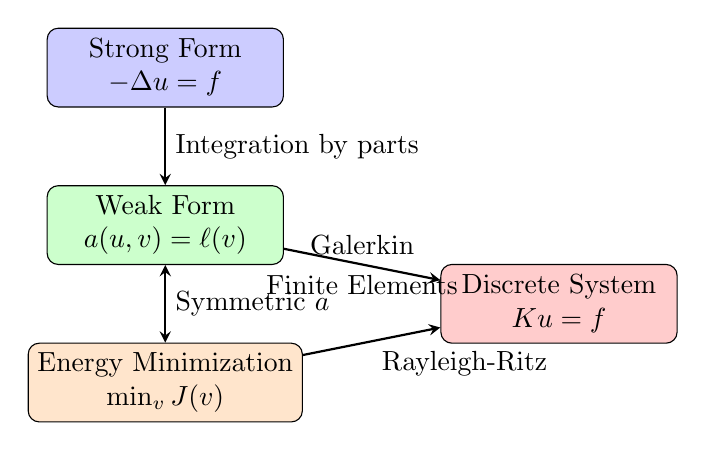
\begin{tikzpicture}[
    box/.style={rectangle, draw, rounded corners, minimum width=3cm, minimum height=1cm, align=center},
    arrow/.style={->, >=stealth, thick}
]
    % Nodes
    \node[box, fill=blue!20] (strong) at (0, 4) {Strong Form \\ $-\lapl u = f$};
    \node[box, fill=green!20] (weak) at (0, 2) {Weak Form \\ $a(u,v) = \ell(v)$};
    \node[box, fill=orange!20] (energy) at (0, 0) {Energy Minimization \\ $\min_v J(v)$};
    \node[box, fill=red!20] (discrete) at (5, 1) {Discrete System \\ $Ku = f$};
    
    % Arrows
    \draw[arrow] (strong) -- node[right] {Integration by parts} (weak);
    \draw[arrow, <->] (weak) -- node[right] {Symmetric $a$} (energy);
    \draw[arrow] (weak) -- node[above] {Galerkin} node[below] {Finite Elements} (discrete);
    \draw[arrow] (energy) -- node[below right] {Rayleigh-Ritz} (discrete);
\end{tikzpicture}
\caption{Connections between different formulations of elliptic PDEs}
\end{figure}

\subsection{Key Theorems Summary}

\begin{center}
\begin{tabular}{lll}
\toprule
\textbf{Theorem} & \textbf{Statement} & \textbf{Numerical Impact} \\
\midrule
Lax-Milgram & Existence \& uniqueness of weak solution & Well-posedness \\
Poincaré & $\norm{u}_{L^2} \leq C_P \norm{\grad u}_{L^2}$ & Condition number \\
Céa's Lemma & $\norm{u-u_h} \leq \frac{M}{\alpha} \inf \norm{u-v_h}$ & Convergence rate \\
\bottomrule
\end{tabular}
\end{center}

\subsection{Why This Matters for Computation}

\begin{enumerate}
    \item \textbf{Well-posedness}: Lax-Milgram guarantees the discrete system has a unique solution
    
    \item \textbf{Error estimates}: Céa's lemma + approximation theory gives $\norm{u - u_h} = \mathcal{O}(h^k)$ for $k$-th order elements
    
    \item \textbf{Condition number}: $\kappa = M/\alpha \sim h^{-2}$ explains why:
    \begin{itemize}
        \item Iterative methods need $\mathcal{O}(h^{-2})$ iterations without preconditioning
        \item Multigrid achieves $\mathcal{O}(n)$ by using multiple scales
    \end{itemize}
    
    \item \textbf{Energy principle}: The solution minimizes a quadratic → the discrete system is SPD → CG is optimal
\end{enumerate}

%=============================================================================
\section*{Appendix: Proof of Key Inequalities}
%=============================================================================

\subsection*{A.1 Cauchy-Schwarz Inequality}

For any inner product space:
\begin{equation}
    |\inner{u}{v}| \leq \norm{u} \cdot \norm{v}
\end{equation}
with equality iff $u$ and $v$ are linearly dependent.

\subsection*{A.2 Young's Inequality}

For $a, b \geq 0$ and $\epsilon > 0$:
\begin{equation}
    ab \leq \frac{\epsilon}{2} a^2 + \frac{1}{2\epsilon} b^2
\end{equation}

This is crucial for deriving coercivity estimates when lower-order terms are present.

\subsection*{A.3 Trace Inequality}

For $u \in H^1(\Omega)$ with smooth $\partial\Omega$:
\begin{equation}
    \norm{u}_{L^2(\partial\Omega)} \leq C_T \norm{u}_{H^1(\Omega)}
\end{equation}

This justifies boundary integrals in the weak formulation.

%=============================================================================
\begin{thebibliography}{9}

\bibitem{evans}
L.C. Evans, \textit{Partial Differential Equations}, 2nd ed., AMS, 2010.

\bibitem{brenner}
S.C. Brenner and L.R. Scott, \textit{The Mathematical Theory of Finite Element Methods}, 3rd ed., Springer, 2008.

\bibitem{ciarlet}
P.G. Ciarlet, \textit{The Finite Element Method for Elliptic Problems}, SIAM Classics, 2002.

\bibitem{braess}
D. Braess, \textit{Finite Elements: Theory, Fast Solvers, and Applications in Solid Mechanics}, 3rd ed., Cambridge, 2007.

\bibitem{hackbusch}
W. Hackbusch, \textit{Elliptic Differential Equations: Theory and Numerical Treatment}, Springer, 2017.

\end{thebibliography}

\end{document}
